\documentclass[tikz,border=4pt]{standalone}
\usepackage[T1]{fontenc}
\usepackage{helvet,amsmath,amssymb}
\renewcommand{\familydefault}{\sfdefault}
\usetikzlibrary{arrows.meta,positioning,fit,calc,shapes.geometric,backgrounds}
\definecolor{navy}{HTML}{193A56}
\definecolor{teal}{HTML}{167D8D}
\definecolor{amber}{HTML}{B87420}
\definecolor{pale}{HTML}{EDF3F6}
\definecolor{mint}{HTML}{EAF5F2}
\definecolor{warm}{HTML}{FFF3E3}
\definecolor{gray}{HTML}{586772}
\tikzset{box/.style={draw=navy!60,rounded corners=2pt,fill=pale,align=center,inner sep=6pt,font=\sffamily\fontsize{8}{9}\selectfont},unit/.style={box,draw=teal,fill=mint},gate/.style={box,draw=amber,fill=warm},arr/.style={-{Latex[length=2.2mm]},thick,draw=navy},note/.style={font=\sffamily\footnotesize,text=gray,align=left},label/.style={font=\sffamily\bfseries\small,text=navy}}
\begin{document}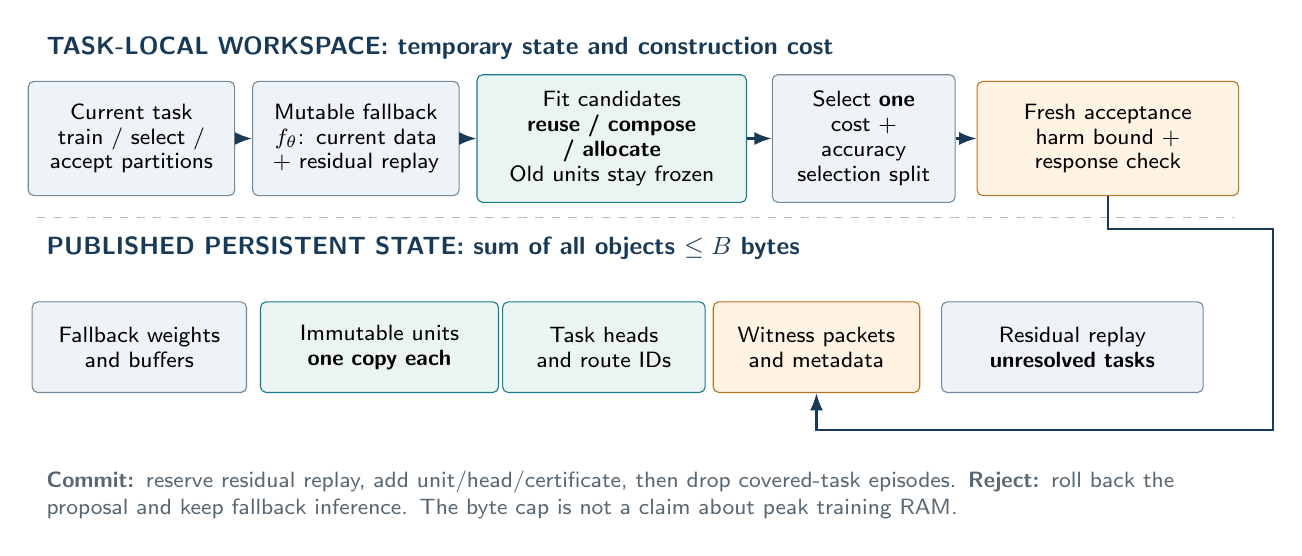
\begin{tikzpicture}[x=1cm,y=1cm]

\node[label,anchor=west] at (0,4.7) {TASK-LOCAL WORKSPACE: temporary state and construction cost};
\node[box,text width=2.2cm,minimum height=1.45cm] (data) at (1.2,3.55) {Current task\\train / select /\\accept partitions};
\node[box,text width=2.2cm,minimum height=1.45cm] (base) at (4.05,3.55) {Mutable fallback\\$f_\theta$: current data\\+ residual replay};
\node[unit,text width=3.0cm,minimum height=1.45cm] (cand) at (7.3,3.55) {Fit candidates\\\textbf{reuse / compose}\\\textbf{/ allocate}\\Old units stay frozen};
\node[box,text width=1.9cm,minimum height=1.45cm] (select) at (10.5,3.55) {Select \textbf{one}\\cost + accuracy\\selection split};
\node[gate,text width=2.9cm,minimum height=1.45cm] (gate) at (13.6,3.55) {Fresh acceptance\\harm bound +\\response check};
\foreach \a/\b in {data/base,base/cand,cand/select,select/gate}\draw[arr] (\a)--(\b);
\draw[draw=navy!35,dashed] (0,2.55)--(15.2,2.55);
\node[label,anchor=west] at (0,2.15) {PUBLISHED PERSISTENT STATE: sum of all objects $\leq B$ bytes};
\node[box,text width=2.3cm,minimum height=1.15cm] (pb) at (1.3,.9) {Fallback weights\\and buffers};
\node[unit,text width=2.6cm,minimum height=1.15cm] (pu) at (4.35,.9) {Immutable units\\\textbf{one copy each}};
\node[unit,text width=2.15cm,minimum height=1.15cm] (ph) at (7.2,.9) {Task heads\\and route IDs};
\node[gate,text width=2.2cm,minimum height=1.15cm] (pc) at (9.9,.9) {Witness packets\\and metadata};
\node[box,text width=2.9cm,minimum height=1.15cm] (pr) at (13.15,.9) {Residual replay\\\textbf{unresolved tasks}};
\draw[arr] (gate.south)--(13.6,2.4)--(15.7,2.4)--(15.7,-.15)--(9.9,-.15)--(pc.south);
\node[note,text width=14.8cm,anchor=north west] at (0,-.55) {\textbf{Commit:} reserve residual replay, add unit/head/certificate, then drop covered-task episodes. \textbf{Reject:} roll back the proposal and keep fallback inference. The byte cap is not a claim about peak training RAM.};
\end{tikzpicture}\end{document}